\documentclass[presentation]{beamer}
\usepackage{graphicx}
\usepackage{longtable}
\usepackage{wrapfig}
\usepackage{rotating}
\usepackage[normalem]{ulem}
\usepackage{amsmath}
\usepackage{amssymb}
\usepackage{capt-of}
\usepackage{hyperref}
\usepackage{esint}
\usepackage{unicode-math}
\usepackage{DejaVuSansMono} % Contains most characters
\usepackage{sourcecodepro} % Bit better looking monospaced with greek letters
\usepackage{tikz}                 % Vector graphics
\usetikzlibrary{arrows.meta,shapes,positioning,tikzmark,decorations.pathmorphing}

\def\aliaser#1#2{%
  % Lowercase trick, store the symbol without tokenizing it just yet
  \begingroup%
  \lccode`~=`#1%
  \lowercase{\endgroup%
    \def~{#2}%
  }%
  \catcode`#1=13%
}
\ExplSyntaxOn % Ignore whitespace, make : _ letters, and ~ a regular space

\usepackage{fontspec}
% Basically the regular tt font but more complete character set
\setmonofont[%
  ItalicFont=NewCMMono10-Italic.otf,%
  BoldFont=NewCMMono10-Bold.otf,%
  BoldItalicFont=NewCMMono10-BoldOblique.otf,%
  SmallCapsFeatures={Numbers=OldStyle}%
]{NewCMMono10-Regular.otf}

\usepackage{minted}[samepage] % Enables source code listings

\catcode`˹=11
\catcode`˺=11
\newminted[LeanCode]{lean4}{frame=single,autogobble,escapeinside=˹˺,fontsize=\small}
\newminted[JsonCode]{json}{frame=single,autogobble,escapeinside=**,fontsize=\small}
\newmintinline[lean]{text}{}
\newminted[HaskellCode]{Haskell}{frame=single,autogobble,escapeinside=**,fontsize=\footnotesize}
\newmintinline[haskell]{text}{}
\newminted[LeanIR]{Lean4}{frame=single,autogobble,fontsize=\small}

\newcommand\unfade{\pgfsetfillopacity{1}\pgfsetstrokeopacity{1}}
\newcommand\fade{\pgfsetfillopacity{0.3}\pgfsetstrokeopacity{0.3}}
\NewDocumentEnvironment{LeanCodeHL}{}{
  \VerbatimEnvironment
  \begingroup
  \aliaser‹\unfade
  \aliaser›\fade
  \fade
  % TODO: escapeinside and gobble don't work together for some unknown reason
  \begin{minted}[escapeinside=˹˺,autogobble]{lean4}
}{
  \end{minted}
  \unfade
  \endgroup
}

\usepackage{newunicodechar}
\makeatletter
\newdimen{\fs}
\def\loanChar#1{
  \newunicodechar{#1}{{
    \fontspec{DejaVuSansMono.ttf}
    % Dejavu is slightly wider than sourcecodepro
    \setlength{\fs}{\f@size pt}\fs=0.996\fs
    \fontsize{\strip@pt\fs}{\strip@pt\dimexpr1.2\fs\relax}\selectfont
    #1
  }}
}
\makeatother

\loanChar{◾}
\loanChar{⟨}
\loanChar{⟩}

% Shorthand for texttt
\newunicodechar{§}{\makeabbreviationtt}
\def\makeabbreviationtt#1§{\texttt{#1}}

\NewDocumentCommand\itemal{O{3cm}mm}{\item ​\hbox to #1{#2\hfill}{#3}}

\ExplSyntaxOff
\usetheme{default}
\author{Nor Führ \& Erik Nygren}
\titlegraphic{
\includegraphics[scale=0.1]{figures/logo.pdf}}
\title{\Huge{Pisa} \\ \Large{Mathematical discovery in Lean}}


\setbeamertemplate{navigation symbols}{}
\hypersetup{
 pdfauthor={},
 pdftitle={Mathematical discovery in Lean},
 pdfkeywords={},
 pdfsubject={},
 pdfcreator={},
 pdflang={English}}
\usemintedstyle{tango}  % a nice, colorful theme

\begin{document}
\frame{\titlepage}

\begin{frame}{Goal} % Pingu
  Create a tool that propose conjectures for a set of existing definitions in Lean.

  \vspace{1cm}

  A focus on transpilation
\end{frame}

% This project, that we call Pisa, set out to try and accomplish a similar goal to that Hipster.
% That is to say, introduce a conjecture generator to Lean based on user provided types and definitions.
% To accomplish this, tooling of Haskell was used, since they had shown their potential with Hipster, and have since gotten more involved in the form of RoughSpec.
% To utilize the tooling from Haskell, a source to source compilation of some form had to be done. So this is the part which we spent most of our time on.

\begin{frame}[fragile]{Usage} % Pingu
  A code action has been created that has the following syntax
  \vspace{1cm}
  \begin{LeanCode}
    #pisa num? ident+
  \end{LeanCode}
\end{frame}

% To begin, lets see how the tool is actually used by people.
% We can see in the slide the code action that was introduced into Lean.
% It shows how it can be used, and we will go through the details later.

% SWITCH TO EMACS BUFFER HERE
% Maybe write binary tree quickly and show new types quickly
 % Pingu
% ~ 1 min
% So heres an overvew of the data flow of the tool.
% From the demo you saw the perspective of the user.
% They interract with the tool through a lean macro.
% This macro sort of orchestrates everything
% So first it retrives relevant information through an exporter
% This information is then passed on to the haskell component that consists of three parts
% ~~~~~~~~~~
% Here the definitions are first translated into Haskell for which conjectures can be generated.
% Those are then translated back into Lean and returned to the macro to be inserted for the user.

% We'll now chronologicaly go into further details

\begin{frame}{How did we do this?} % Kiren
\begin{figure}
  \centering
  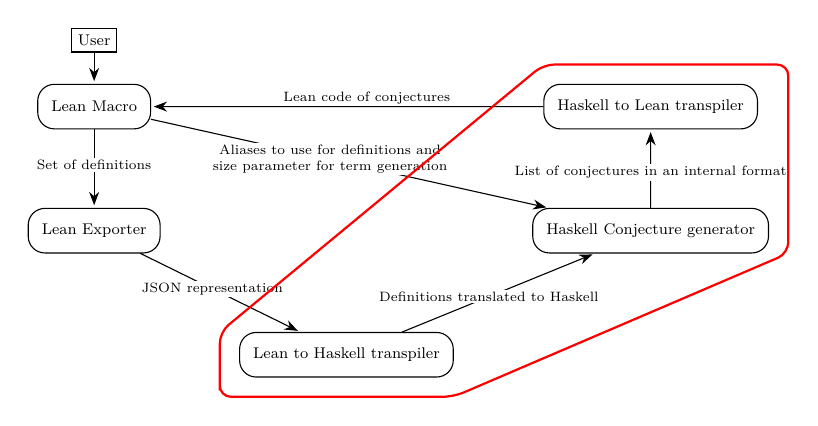
\begin{tikzpicture}[font=\footnotesize, ->, >={Stealth[sep]}, scale=0.7, every node/.style={scale=0.7}]
    \tikzstyle{module} = [rectangle, draw, rounded corners=6, inner sep=7, minimum height=23]
    \tikzstyle{desc} = [pos=0.45, fill=white, font=\scriptsize, align=center, inner sep=1]

    \node[draw]                          (us)  {User};
    \node[module, below      =0.4 of us] (lm)  {Lean Macro};
    \node[module, below      =of lm]     (ex)  {Lean Exporter};
    \node[module, below right=of ex]     (l2h) {Lean to Haskell transpiler};
    \node[module, above right=of l2h]    (cg)  {Haskell Conjecture generator};
    \node[module, above      =of cg]     (h2l) {Haskell to Lean transpiler};

    \draw (us)  -- (lm);
    \draw (lm)  -- (cg)  node[desc]        {Aliases to use for definitions and \\ size parameter for term generation};
    \draw (lm)  -- (ex)  node[desc]        {Set of definitions};
    \draw (ex)  -- (l2h) node[desc]        {JSON representation};
    \draw (l2h) -- (cg)  node[desc]        {Definitions translated to Haskell};
    \draw (cg)  -- (h2l) node[desc]        {List of conjectures in an internal format};
    \draw (h2l) -- (lm)  node[desc, above,fill=none] {Lean code of conjectures};

    \pause
    \draw[draw=gray, rounded corners, thick, draw=red, -]
      ([xshift=1em, yshift=1em]h2l.north east) -|
      ([xshift=1em]cg.south east) --
      ([yshift=-1em]l2h.south east) -|
      ([xshift=-1em, yshift=-1em]l2h.south west) -|
      ([xshift=-1em]l2h.north west) --
      ([yshift=1em]h2l.north west) --
      ([xshift=1em, yshift=1em]h2l.north east);
  \end{tikzpicture}
\end{figure}
\end{frame}
 % Kiren
\section{Lean}\label{sec:lean}
Lean is a dependently typed functional programming language that is combined with text editor plugins to make a proper interactive theorem prover (ITP).
In this thesis Lean refers specifically to the latest version, Lean 4.
It is significantly more extensible than earlier iterations and features a compiler that is able to generate relatively efficient C code \autocite{Lean4}.
The efficient compiler has enabled it to be mostly bootstrapped, however, the kernel used for verification is yet to be ported from \cpp.

Three of the concepts utilized by Lean are of particular relevance to this thesis.
First, a typed lambda calculus that relates to the source code, encodes definitions, and the types of definition \autocite{Declaration}.
The lambda calculus allows for type checking and reductions.
Second, a kernel that is a small, trusted computing base.
The kernel is used for verification of correctness for Lean programs.
The reason why it is small is so that it should itself be verifiable, in order to trust its output.
Third, an intermediate representation (IR) which is used for compilation of programs, that allows for evaluation of statements or running entire programs \autocite{IR}.

\subsection{Example of syntax}
Familiarity with Lean syntax may help to better understand parts of this thesis.
The examples that follows should give a sense of the syntax used in some Lean listings.
However, syntax in Lean is very extensible as will be explained later, and the same code may be written in multiple ways.

\paragraph*{Algebraic data types} can be defined as in \cref{lst:syntax:inductives}.
The start of such a declaration use the keyword \lean{inductive}, which signifies a type that induction can be done on.
Booleans are, for example, defined as the sum of two trivial values, §t§ and §f§ representing true and false respectively.
Each variant of the sum is syntactically initiated by a vertical bar followed by its name and type.

\begin{listing}[ht]
\begin{LeanCode}
inductive B where | t : B | f : B

inductive P where | p : B → B → P

inductive N where | z : N | s : N → N

inductive L : Type → Type where
  | Nil : L α
  | Cons : α → L α → L α
\end{LeanCode}
\caption{Example of inductive types declared in Lean.}
\label{lst:syntax:inductives}
\end{listing}

All inductives in Lean are a sum of product types.
In the second definition a product type, §P§, is exemplified by adding premises, or arguments, to the variant type.
In an inductive definition these arguments may be of the type that is constructed, as shown by §N§.
Here, natural numbers are defined recursively as in the Peano axioms; a zero, §Z§, is trivially constructed, and by providing any number $n$ a successive number $n+1$ is constructed with §S n§.

A type itself may be parametric, that is to say the type itself takes arguments in the form of types.
The final example in \cref{lst:syntax:inductives} demonstrates a definition of a polymorphic list, which takes a type as an argument.
In this definition the given type is referred to by a free variable, §α§, that will be resolved by Lean from the context where the constructors are used.
In \lean{Cons t Nil} the type can be inferred to lists of Booleans since the first argument to §Cons§ is a boolean, which is consistent with §Nil§ since it is a list of any type.

\paragraph*{Definitions} associate any expression with a name.
Some examples are given in \cref{lst:syntax:def}.
Since types are ostensibly values of the type §Type§ there is no strict distinction between values and types.
Thus, what would be defined as a type alias in languages such as Haskell where values and types are distinguished, is a regular definition, such as the example \lean{NatList}.
However for this thesis, definitions are typically functions, which is shown in the three last §def§ in \cref{lst:syntax:def}.

Case matching on types is done in two different ways: one where it is specified what is matched on, as can be seen in \lean{not} and \lean{add}, and the other where the case can be done instead of a lambda, which is seen in \lean{sum}.
The dot seen before the constructors in the §match§ is to avoid opening the inductive types scope, that is to say adding the constructor as a function in the current context.
The way Lean finds the right constructor using the dot syntax is by looking through the context for a constructor with that name and type.

\begin{listing}[ht]
\begin{LeanCode}
def NatList := L N

def not (b : B) :=
  match b with | .t => .f | .f => .t

def add : N → N → N := λ n m =>
  match m with | .Z => n | .S m' => .S (add n m')

def sum : NatList → N
  | .Nil => .Z
  | .Cons a as => add a (sum as)
\end{LeanCode}
\caption{Example of how definitions can be declared in Lean.}
\label{lst:syntax:def}
\end{listing}

\paragraph*{Theorems} are a special case of regular definitions that are used when proving propositions.
The truth value of a proposition is proven by having a resulting type that is a §Prop§.
Reflexivity or equality, is the proposition that is relevant for the conjectures generated by Pisa.
Reflexivity states that the left and right hand sides are definitionally equivalent and has a special syntax which is \lean{lhs = rhs}~\autocite{rfl}.
The example in \cref{lst:syntax:thm} is a theorem proving that \lean{not (not b)} is equivalent to \lean{b}.
This verified by the type checker, ensuring that both potential cases of §b§ resolve to the same definition.
In the case where \lean{b = .t}, \lean{not (not .t)} resolves to §.t§, and is therefore being able to construct §rfl§ (§rfl§ is one of the constructors of properties).
Theorems are the basis of using Lean as a proof engine, since the resulting type should be a truthful statement.

\begin{listing}[ht]
\begin{LeanCode}
theorem not_not (b : B) : not (not b) = b :=
  match b with | .t => rfl | .f => rfl
\end{LeanCode}
\caption
  [Example of a theorem proving elimination of double negations.]
  {Example of a theorem in Lean. In this case proving elimination of double negations by constructing a reflexivity value.}
\label{lst:syntax:thm}
\end{listing}

\subsection{Extensible syntax}\label{sec:lean:extensible-syntax}
A central feature of Lean is that the parser may be extended by the code that itself is parsing \autocite{LeanMacros}.
This is a more generalized approach to syntactic sugar supported by many other languages, including Lean 3.
By supporting arbitrary syntax Lean can embed domain specific languages appropriate for the context in which a proof is developed.
This greatly improves usability as an ITP.

The core idea to this extensibility is to quantify syntax elements and their rules, which is done through syntactic categories, e.g. identifiers, terms, or commands.
Additional new categories may be devised, and any category can be extended with syntax rules.
There are two kinds of rules, \textit{macros} and \textit{elaborators}.
A macro transforms syntax into other syntax, which in turn may be described by another macro.
When no macros are applicable to a piece of syntax it is finally evaluated by a matching elaborator.
These produce computations with side effects, that have access to the internal compiler state.

Elaborators enable context aware syntax.
An example provided by~\cite{Elaborators}, is the syntax \lean{a !: b}, which means that §a§ will only evaluate if it is not of the type §b§.
In \cref{lst:extensible:not}, §!:§ allows the compiler to verify that the first term is not of a certain type, even if it depends on a larger context.

\begin{listing}[ht]
\begin{LeanCode}
#eval ([1, 2, 3] !: String) -- Evaluates to [1,2,3]
#eval (5 !: Nat) -- Fails type checking due to 5 being of the type Nat
\end{LeanCode}
\caption
  [Example of extensible syntax in Lean.]
  {Example of extensible syntax, which elaborates a term to a different term that may or may not type check.}
\label{lst:extensible:not}
\end{listing}

Elaboration produces expressions for the Lean kernel, that may either be evaluated for soundness or transformed into executable code.
The former relying on the typed lambda calculus, and the latter on the IR, both described in the following sections.

% \subsection{Language server}\label{sec:lean:lsp}

\subsection{Typed lambda calculus}\label{sec:lean:typed-lambda-calculus}
Lean has a dependently typed lambda calculus that is used for type checking which enables the use of dependent types \autocite{Lean}.
It has fundamental declarations, but the main ones that are used for this thesis are §definitional§, §constructor§, §inductive§ and §recursor§ values.
These all explain different aspects of the language, where §constructor§ is the explanation of how the constructor works, §inductive§ for data types, §definitional§ for definitions (such as functions), and §recursor§ for how recursion is done on inductives \autocite{Declaration}.
All the before mentioned, have a type, which is an expression.

Expressions are the lambda calculus in action.
The lambda expressions have the standard application, lambda, and variable constructors one would expect.
The lambda expressions use de Bruijn Indices, which uses numbers to represent what binder a variable references.\footnote{There also exists free and meta variables that do not use de Bruijn Indices.}
Worth of note, is the constructor \lean{Const}.
\lean{Const} is how definitions are mentioned, for example in an application, in the current definition.

The §recursor§ value is used to represent mathematical induction on §inductive§ types.
A set of functions are auto generated for each inductive type to use this. An example of an auto generated function is \lean{.rec}.
\lean{.rec} is a unique part of the language, that is based on the structure of its inductive counterpart.
This enables higher level concepts such as case matching and recursion to be simple to represent.
Using the natural numbers as an example, as can be seen in \cref{lst:recursor}.
The first argument of \lean{.rec} is the §motive§, which there may be more than of depending on what criteria is needed for recursion.
The §motive§ is what the resulting operation should resolve to, for example a boolean.
In the case of a boolean the motive would look like the following: \lean{motive : N → B}.
Following this is how the cases should result in different resulting values.
Last, is the value that recursion is performed on.
The return type of \lean{.rec} is dependent on the motive, as mentioned, therefore, the §motive§ is applied to the value, to figure out what the resulting type is.

\vspace{-0.4cm}
\begin{listing}[H]
\begin{LeanCode}
inductive N where
  | Z : N
  | S : N → N

N.rec {motive : N → Type}
      (Z : motive Z)
      (S : (a : N) → motive a → motive (S a))
      (t : N) :
      motive t
\end{LeanCode}
\caption
  [Pseudo Lean code demonstrating the auto generated function §.rec§.]
  {Pseudo Lean code demonstrating how the auto generated function §.rec§ is added to natural numbers.}
\label{lst:recursor}
\end{listing}

\subsection{Intermediate representation}\label{sec:lean:intermediate-representation}
To construct efficient C code Lean definitions are transformed into an intermediate representation (IR).
This additionally enables efficient interactive evaluation of Lean code.
Built into Lean is a provided command \lean{#eval}.
\lean{#eval} is used to evaluate most Lean expressions, similar to an external interpreter but within the document editor.
For example, \lean{#eval 4 + 4} would, as one would expect, print §8§.

The IR of Lean is based on \λ{Pure} and \λ{Rc}, explained in \citetitle{Beans} by~\cite{Beans}.
The IR could be seen through the lens of C; it deals with a list of sequential instructions and branches of instructions.
All values are represented by the following types, described by~\cite{IR}:
\vspace{-0.2cm}
\begin{multicols}{4}
\begin{itemize}[noitemsep]
    \item float
    \item uint8
    \item uint16
    \item uint32
    \item uint64
    \item usize
    \item irrelevant
    \item object
    \item tobject
    \item float32
    \item struct
    \item union
\end{itemize}
\end{multicols}
\vspace{-0.2cm}

For this thesis, values in Lean will usually be encoded as a constructor, based on an §inductive§ tagged with an identifying type.
In \cref{lst:ir}, \lean{n} would be encoded as a constructor with the tag $1$ due to being the second constructor in the inductive type.
\lean{n} would then have a pointer to the sub constructor \lean{S(Z)} in its list of values associated to the constructor.
\begin{listing}[H]
\begin{LeanCode}
inductive N where
  | Z : N
  | S : N → N

-- zero =           Constructor (Tag 0) []
-- one  =           Constructor (Tag 1) [zero]
def n := S(S(Z)) -- Constructor (Tag 1) [one]
\end{LeanCode}
\caption[Illustration of the IR representation for inductive Lean values.]{
  Illustration of the IR representation for some Lean values.
  Numbers constructed using an inductive Peano definitions with comments showing their respective IR representation.
}
\label{lst:ir}
\end{listing}

\vspace{-0.4cm}
In contrast to how \cref{lst:ir} would be encoded, values of \lean{B} in \cref{lst:ir2} would be encoded as an unsigned integer.
Since no constructor in \lean{B} requires any arguments, it is interpreted as an enum, since it only needs a tag.
\lean{true} would therefore be encoded to a $0$, and \lean{false} as $1$.

\begin{listing}[H]
\begin{LeanCode}
inductive B where
  | t : B
  | f : B

def true  := .t -- 0 : uint8
def false := .f -- 1 : uint8
\end{LeanCode}
\caption
  [Illustration of the IR representation for enumerated Lean values.]
  {Illustration §true§ and §false§ encoding the Boolean value for true and false and comments with their respective IR representation.}
\label{lst:ir2}
\end{listing}
 % Kiren
% ~2 min
% And that's that for the lean part so far.
% The exported data is now piped to the haskell executable and deserialized.
% This is where the main focus of our work happens.
% - Transpiling the Lean code to Haskell
% ~~~~~~~~
% There are two aspects to the transpilation that are handled a bit differently.
% Data types and their constructors for one
% And second, other definitions, mainly functions.
% ~~~~~~~~
% For data types there is a pretty straight forward corespondence between the languages
% as is demonstrated by this list-like data type.
% This is however somewhat fragile.
% In Haskell types and values live in two separate worlds,
% whereas in Lean types can depend regular values and are themselves regular values
% But for the scope of our tool, this difference is not accounted for.
% ~~~~~~~~
% The actual exported representation is more akin to this snipet.
% The important difference here is that the variable alpha is not shared between the definitions
% ~~~~~~~~
% So here's the same definition showcasing their independence
% But in the generated Haskell code this is not permitted
% So first we must homonogize these definitons by renaming and removing the type variable
% ~~~~~~~~
% When that is done, we simply have to be able to translate these type signatures
% Which happened to be pretty straight forward.
% ~~~~~~~~
% Finally, to help the conjecture generator abstractly represent arbitrary polymophism
% we have replace the type variable with a specific type called `Poly`
% What proved to not be as straight forward as this is translating regular definitions.

\begin{frame}{Lean to Haskell Transpiler} % Kiren
\begin{figure}
  \centering
  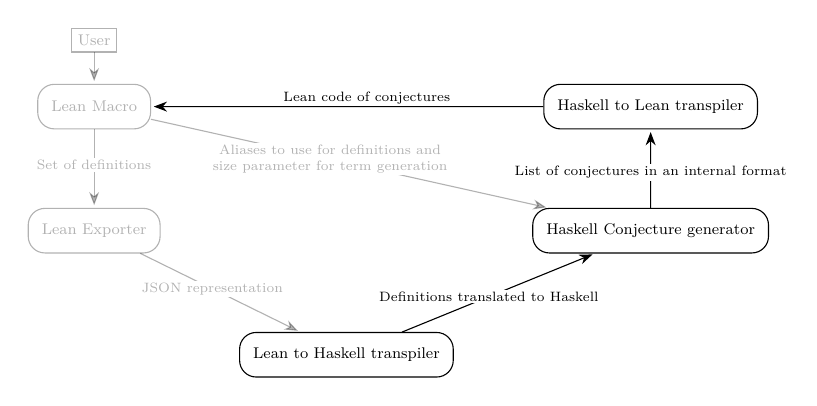
\begin{tikzpicture}[font=\footnotesize, ->, >={Stealth[sep]}, scale=0.7, every node/.style={scale=0.7}]
    \tikzstyle{module} = [rectangle, draw, rounded corners=6, inner sep=7, minimum height=23]
    \tikzstyle{desc} = [pos=0.45, fill=white, font=\scriptsize, align=center, inner sep=1]
    \tikzstyle{fesc} = [text opacity= 0.3, fill opacity=1, desc]

    \fade
    \node[draw]                          (us)  {User};
    \node[module, below      =0.4 of us] (lm)  {Lean Macro};
    \node[module, below      =of lm]     (ex)  {Lean Exporter};
    \unfade
    \node[module, below right=of ex]     (l2h) {Lean to Haskell transpiler};
    \node[module, above right=of l2h]    (cg)  {Haskell Conjecture generator};
    \node[module, above      =of cg]     (h2l) {Haskell to Lean transpiler};

    \fade
    \draw (us)  -- (lm);
    \draw (lm)  -- (cg)  node[fesc]        {Aliases to use for definitions and \\ size parameter for term generation};
    \draw (lm)  -- (ex)  node[fesc]        {Set of definitions};
    \draw (ex)  -- (l2h) node[fesc]        {JSON representation};
    \unfade
    \draw (l2h) -- (cg)  node[desc]        {Definitions translated to Haskell};
    \draw (cg)  -- (h2l) node[desc]        {List of conjectures in an internal format};
    \draw (h2l) -- (lm)  node[desc, above] {Lean code of conjectures};
  \end{tikzpicture}
\end{figure}
\end{frame}

\begin{frame}{Lean to Haskell Transpiler} % Kiren
  Two aspects

  \begin{itemize}
  \item Data types \& Constructors
  \item Definitions: Functions
  \end{itemize}

\end{frame}

\begin{frame}[fragile]{Lean to Haskell Transpiler: Data types \& Constructors} % Kiren
  % \begin{LeanCode}
  %   inductive B where | t :  B | f :  B
  % \end{LeanCode}
  % \begin{HaskellCode}
  %   data      B where ; T :: B ; F :: B
  % \end{HaskellCode}

  \begin{overprint}
    \onslide<1-2>
    \begin{columns}[T]
      \begin{column}{.48\textwidth}
        \begin{LeanCode}
          inductive L α
            where
            | Nil : L α
            | Cons : α → L α → L α
        \end{LeanCode}
        \centering
        Lean version
      \end{column}
      \begin{column}{.48\textwidth}
        \begin{HaskellCode}[fontsize=\small]
          data L α
            where
            Nil :: L α
            Cons :: α -> L α -> L α
        \end{HaskellCode}
        \centering
        Haskell version
      \end{column}
    \end{columns}
    \onslide<3-4>
    \begin{columns}[T]
      \begin{column}{.48\textwidth}
        \begin{LeanCode}
          inductive L : Type → Type
            where
            | Nil : L β
            | Cons : γ → L γ → L γ
        \end{LeanCode}
        \centering
        Lean version
      \end{column}
      \begin{column}{.48\textwidth}
        \begin{HaskellCode}[fontsize=\small]
          data L α
            where
            Nil :: L α
            Cons :: α -> L α -> L α
        \end{HaskellCode}
        \centering
        Haskell version
      \end{column}
    \end{columns}
    \onslide<5>
    \begin{columns}[T]
      \begin{column}{.48\textwidth}
        \begin{LeanCode}
          inductive L : Type → Type
            where
            | Nil : L β
            | Cons : γ → L γ → L γ
        \end{LeanCode}
        \centering
        Lean version
      \end{column}
      \begin{column}{.48\textwidth}
        \begin{HaskellCode}[fontsize=\small]
          data L Poly where
            Nil :: L Poly
            Cons :: Poly -> L Poly
                         -> L Poly
        \end{HaskellCode}
        \centering
        Haskell version
      \end{column}
    \end{columns}
  \end{overprint}

  \vspace{1cm}
  \begin{columns}[T]
    \begin{column}{.65\textwidth}
  \begin{overprint}
    \onslide<2>
    \begin{LeanCode}
      L := Type → Type
      L.Nil := (α : Type) → L α
      L.Cons := (α : Type) → α → L α → L α
    \end{LeanCode}
    \onslide<3>
    \begin{LeanCode}
      L := Type → Type
      L.Nil := (β : Type) → L β
      L.Cons := (γ : Type) → γ → L γ → L γ
    \end{LeanCode}
    \onslide<4->
    \begin{LeanCode}
      L := (α : Type) → Type
      L.Nil := L α
      L.Cons := α → L α → L α
    \end{LeanCode}
  \end{overprint}
      \end{column}
    \end{columns}
  \bigskip
  \begin{overprint}
    \onslide<2-3>
    \begin{center}
      Exported representation
    \end{center}
  \end{overprint}
\end{frame}

\begin{frame}[allowframebreaks,fragile]{Lean to Haskell Transpiler: Functions} % Pingu
  Intermediate representation used by Lean

  % So, a question that arises when using lean is how it evaluates expressions in the editor.
  % Short answer, using an IR that gets converted to C code, and is then evaluated.
  % What if, you can export the first iteration of this IR?
  % Turns out, you can

  \framebreak
  \begin{columns}[T]
    \begin{column}{.48\textwidth}
      \begin{LeanCode}
        inductive B where
          | t : B
          | f : B

        def not (b : B) : B :=
          match b with
          | .t => .f
          | .f => .t
      \end{LeanCode}
      \centering
      Lean version
    \end{column}
    \begin{column}{.48\textwidth}
      \begin{LeanIR}
        def not (x_1 : u8) : u8 :=
          case x_1 : u8 of
          B.t →
            let x_2 : u8 := 1;
            ret x_2
          B.f →
            let x_3 : u8 := 0;
            ret x_3
      \end{LeanIR}
      \centering
      IR version
    \end{column}
  \end{columns}

  % Here, we can see an example of the conversion between the Lean code and IR for the function not
  % It is quite similar, but worth noting is that the Boolean has been converted into an number, representing the index it held in the enum.
  % The IR tries to do these optimizations, even in the first iteration, since they allow for leaner (haha) code.

  \framebreak
  \begin{LeanCode}
  inductive L (α : Type) where
    | Nil : L α
    | Cons : α → L α → L α

  def append {α : Type} (xs : L α) (ys : L α) : (L α) :=
    match xs with
    | .Nil => ys
    | .Cons a as => .Cons a (append as ys)
  \end{LeanCode}

  % So what if, we have a more complicated example, such as append for lists.
  % There is polymorphism, and recursion in this, how does the IR handle it?

  \framebreak

  \begin{minted}[frame=single,autogobble,fontsize=\tiny]{Lean4}
  def append._rarg (x_1 : obj) (x_2 : @& obj) : obj :=
    case x_1 : obj of
    L.Nil →
      inc x_2;
      ret x_2
    L.Cons →
      let x_3 : u8 := isShared x_1;
      case x_3 : u8 of
      Bool.false →
        let x_4 : obj := proj[1] x_1;
        let x_5 : obj := append._rarg x_4 x_2;
        set x_1[1] := x_5;
        ret x_1
      Bool.true →
        let x_6 : obj := proj[0] x_1;
        let x_7 : obj := proj[1] x_1;
        inc x_7;
        inc x_6;
        dec x_1;
        let x_8 : obj := append._rarg x_7 x_2;
        let x_9 : obj := ctor_1[L.Cons] x_6 x_8;
        ret x_9
  def append (x_1 : ◾) : obj :=
    let x_2 : obj := pap append._rarg._boxed;
    ret x_2
  def append._rarg._boxed (x_1 : obj) (x_2 : obj) : obj :=
    let x_3 : obj := append._rarg x_1 x_2;
    dec x_2;
    ret x_3
  \end{minted}

  % The append function is ''just`` 2 lines.
  % But what is this black box?
  % And how does the _rarg work?
  % Well, the box is to allow for partially applied functions in a special way, and is named irrelevant.
  % It is done to allow for the boxing aspect, since the IR is based on Lambda RC which allows for mutable data.
  % And the actually applied values will be of the object type

  \framebreak

  What about values then?

  % Values are how IR handles, and for most of the types used, will usually either become objects, or enums.

  \framebreak

  \begin{HaskellCode}
    data Object = Object { rc :: Int, tag :: Natural }

    data Val
      = Unsigned Natural
      | ** ...**
      | VCtor { o :: Object, vs :: [Val] }

    fromValPoly :: Val -> Poly
    fromValPoly = \case
      Unsigned a -> Poly a

    toValPoly :: Poly -> Val
    toValPoly (Poly a) = Unsigned a
  \end{HaskellCode}

  % Here we can see the encoding of the different values, but since we need to be able to autogenerate the datatypes explained by Erik earlier, the Poly type was introduced to handle the case for conversion to naturals here.

  \framebreak

  \begin{HaskellCode}
    data L where
      Nil  :: L
      Cons :: Poly -> L -> L

    toValL :: L -> Val
    toValL = \a -> case a of
      Nil -> VCtor (Object 1 0) []
      Cons b c ->
        VCtor (Object 1 1) [toValPoly b, toValL c]

    fromValL :: Val -> L
    fromValL = \(a :: Val) -> case a of
      VCtor (Object _ 0) [] -> Nil
      VCtor (Object _ 1) [b, c] ->
        Cons (fromValPoly b) (fromValL c)
  \end{HaskellCode}

  % So each datatype that we introduce will have to create two functions.
  % One from Val and one to Val.
  % In the case of Lists, we utilize the Poly type to make it monomorphic.

\end{frame}

\begin{frame}[allowframebreaks,fragile]{Conjecture generation} % Pingu
  Get signatures of the roots

  Apply QuickSpec \& RoughSpec

  % So, we have the roots, as given by the user, and we have generated code to evaluate them.
  % Time to plop them into a list for QuickSpec and RoughSpec to generate conjectures on.
  % The signatures will be the name, and how to call them.
  % QuickSpec and RoughSpec will then create different combinations of the specified signatures, and test if they hold up.
  % If a case fails, that is tossed, otherwise they are kept as potential laws and presented to user.

  \pagebreak

  \begin{HaskellCode}
  environment :: Map Name Decl
  environment = fromList [**...**]

  append = FDecl {**...**}

  sigs :: [Sig]
  sigs =
    [ monoType ((Proxy :: Proxy L))
    , con "append"
        (\ a b -> fromValL
          (eval append environment
            [toValL a, toValL b]
          )
        )
    ]
  \end{HaskellCode}

  \pagebreak

  \begin{minted}[frame=single, autogobble]{Output}
  == Laws ==
    1. append (append x y) z = append x (append y z)
  \end{minted}

  % Here we can see an example of what would be expected if only the append function is supplied.
  % And this is the associativity law, which would be expected.

\end{frame}

\begin{frame}[allowframebreaks,fragile]{Reverse translation} % Pingu
  The names of functions can be preserved

  The types need to be kept in a map

  \pagebreak

  \begin{minted}[frame=single, autogobble, fontsize=\footnotesize]{Lean}
  (x y z : T0'L) : append (append x y) z = append x (append y z)
  \end{minted}
  \fade
  \begin{minted}[frame=single, autogobble, fontsize=\footnotesize]{Lean}
  (x y z : L α)  : append (append x y) z = append x (append y z)
  \end{minted}

  \pagebreak

  \fade
  \begin{minted}[frame=single, autogobble, fontsize=\footnotesize]{Lean}
  (x y z : T0'L) : append (append x y) z = append x (append y z)
  \end{minted}
  \unfade
  \begin{minted}[frame=single, autogobble, fontsize=\footnotesize]{Lean}
  (x y z : L α)  : append (append x y) z = append x (append y z)
  \end{minted}

  % Worth of note is that the names of the functions will not always match up with the ones that can be seen for the user in the editor.
  % But when constructing the signatures, replacement names can be provided, which override the internal names.
  % That is great for us, but the names of types are not.
  % So a mapping between the internal Haskell name and the Lean name is kept for reversing it when sent back to the Lean part.
\end{frame}
 % Pingu
\begin{frame}[fragile]{Macro} % Kiren
  \begin{figure}
    \centering
    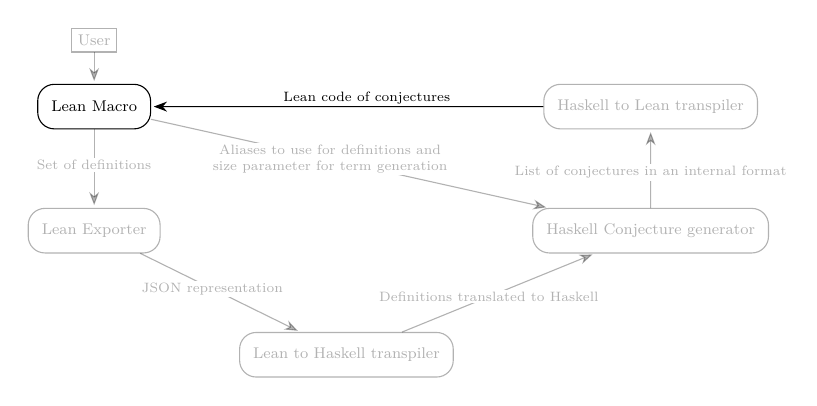
\begin{tikzpicture}[font=\footnotesize, ->, >={Stealth[sep]}, scale=0.7, every node/.style={scale=0.7}]
      \tikzstyle{module} = [rectangle, draw, rounded corners=6, inner sep=7, minimum height=23]
      \tikzstyle{desc} = [pos=0.45, fill=white, font=\scriptsize, align=center, inner sep=1]
      \tikzstyle{fesc} = [text opacity= 0.3, fill opacity=1, desc]

      \fade
      \node[draw]                          (us)  {User};
      \unfade
      \node[module, below      =0.4 of us] (lm)  {Lean Macro};
      \fade
      \node[module, below      =of lm]     (ex)  {Lean Exporter};
      \node[module, below right=of ex]     (l2h) {Lean to Haskell transpiler};
      \node[module, above right=of l2h]    (cg)  {Haskell Conjecture generator};
      \node[module, above      =of cg]     (h2l) {Haskell to Lean transpiler};
      \unfade

      \fade
      \draw (us)  -- (lm);
      \draw (lm)  -- (cg)  node[fesc]        {Aliases to use for definitions and \\ size parameter for term generation};
      \draw (lm)  -- (ex)  node[fesc]        {Set of definitions};
      \draw (ex)  -- (l2h) node[fesc]        {JSON representation};
      \draw (l2h) -- (cg)  node[fesc]        {Definitions translated to Haskell};
      \draw (cg)  -- (h2l) node[fesc]        {List of conjectures in an internal format};
      \unfade
      \draw (h2l) -- (lm)  node[desc, above] {Lean code of conjectures};
    \end{tikzpicture}
  \end{figure}
  \smallskip
  \begin{LeanCode}
    let conjecturesText ← IO.spawn "pisa" =<< export is
  \end{LeanCode}
\end{frame}

\setbeamercovered{transparent}
\begin{frame}{Alternatives approaches} % Kiren
  \begin{itemize}[<+>]
    \item Instantiations of polymorphism
    \item Proof generation
    \item Proper translation using reductions
    \item Performance
    \item Plausible
  \end{itemize}
\end{frame}
 % Kiren

\end{document}
